\section{Experimental Evaluation and Results}
\begin{figure*}[!t]
\centering
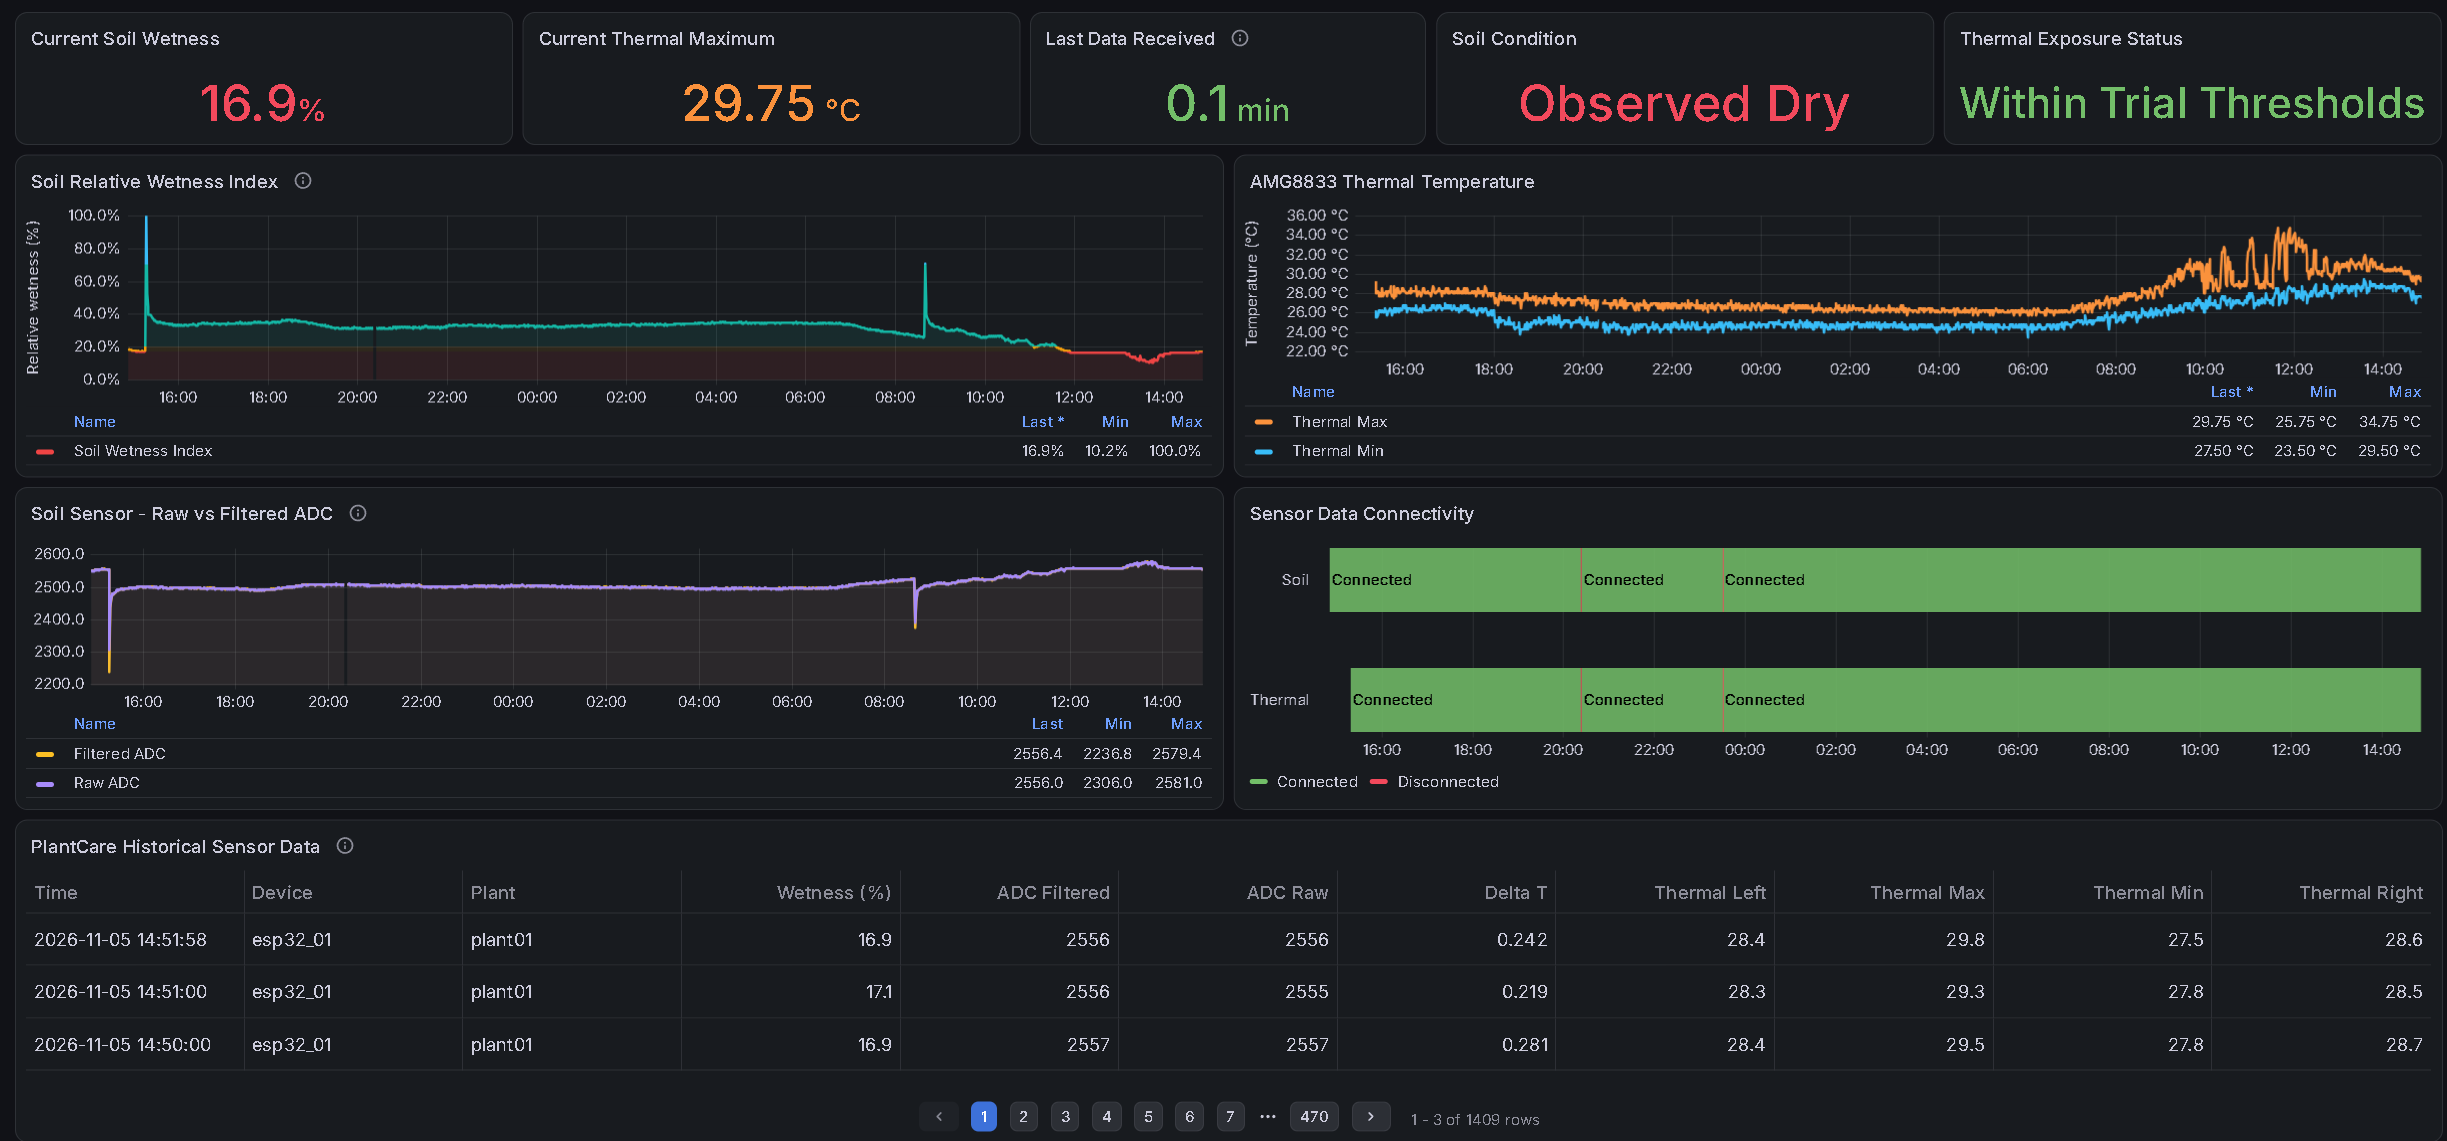
\includegraphics[width=.86\textwidth]{grafana.png}
\caption{Updated Grafana capture from 5 November 2026 showing current readings, both status cards, sensor timelines, and historical rows. The crop removes the browser address and controls.}
\label{fig:grafana}
\end{figure*}
\subsection{Trial Setup and Observed Soil Response}
The observational trial used one hanging pot and the photographed thermal viewing arrangement. The assessment combines before/after snapshots from the ESP32 dashboard, firmware and flow artifacts, a saved Grafana Explore export, and dashboard captures \cite{projectevidence}. The historical export represents one device and plant. The record audit uses the timestamps as printed because the CSV has no UTC offset. Network conditions, power interruptions, and server load were not instrumented.

The exported ingest function passed eight offline checks using a synthetic key and fixture payloads. Soil-only and combined requests returned \code{202}. Invalid key, malformed JSON, wrong device, out-of-range ADC, short thermal frame, and empty sensor payload returned their expected errors and emitted no write messages. The combined fixture used half-frame means of $26\degc$ and $29\degc$ and returned $\Delta T=3\degc$. This exercise covered function behavior without making network requests or measuring write reliability.

Table~\ref{tab:watering} shows four paired observations. The paired mean ADC fell from 2,614 to 2,273.5, a difference of 340.5 counts. The firmware rounds the wet endpoint to 2,274. Every immediate post-watering value is lower than its paired initial value. In the 20 October sequence the reading subsequently rose to 2,501 at 18:24 and 2,522 at 18:57. The sequence supports a short-term sensor response in this pot. The observations lack controlled water volumes, a reference moisture measurement, and independent replicate pots.

\begin{table}[!t]
\caption{Raw ADC before and immediately after manual watering, transcribed from local dashboard captures.}
\label{tab:watering}
\centering\footnotesize
\begin{tabular}{@{}lrrr@{}}
\hline
Observation & Before & After & Drop\\ \hline
20 Oct., evening & 2770 & 2307 & 463\\
21 Oct., morning & 2622 & 2238 & 384\\
21 Oct., evening & 2559 & 2226 & 333\\
22 Oct., morning & 2505 & 2323 & 182\\ \hline
Mean & 2614 & 2273.5 & 340.5\\ \hline
\end{tabular}
\end{table}

\subsection{CSV Completeness and Data Gaps}
The Grafana Explore file saved on 3 November 2026 covers displayed timestamps from 29 October at 09:54 through 3 November at 17:00. A CSV parser counted 5,860 data rows after the header and found 5,860 distinct timestamp, device, and plant keys. All rows have the three soil fields. Of these, 5,844 have all five thermal fields and 16 lack all thermal fields. Thus 99.7\% of exported rows contain both measurement families. A pivoted table row can combine multiple fields and measurements at one minute. Raw InfluxDB points and scheduled archive rows must be counted separately. The Explore CSV has no data-source tag column.

\begin{table}[!t]
\caption{Recounted Grafana Explore rows by displayed date. The first and last dates are partial.}
\label{tab:daily}
\centering\footnotesize
\begin{tabular}{@{}lrrr@{}}
\hline
Date in 2026 & Rows & With soil & With thermal\\ \hline
29 Oct. & 823 & 823 & 823\\
30 Oct. & 1369 & 1369 & 1369\\
31 Oct. & 1340 & 1340 & 1340\\
1 Nov. & 872 & 872 & 872\\
2 Nov. & 1396 & 1396 & 1380\\
3 Nov. & 60 & 60 & 60\\ \hline
Total & 5860 & 5860 & 5844\\ \hline
\end{tabular}
\end{table}

Comparing adjacent timestamps found 141 separations longer than one minute. The largest were 967 minutes (2 November at 23:52 to 3 November at 15:59), 581 minutes (31 October at 23:05 to 1 November at 08:46), and 34 minutes (30 October at 13:05 to 13:39). Across the inclusive export span, 5,860 of 7,627 nominal minute slots appear (76.8\%). The 1,767 absent slots describe this file's coverage. Device downtime, Wi-Fi or TLS failure, ingestion failure, or export query behavior could each produce missing rows. Attribution requires correlated timestamps from firmware, ingest, and database logs.

\subsection{Grafana Visualization and Status Thresholds}
Figure~\ref{fig:grafana} shows a soil index of 16.9\%, a thermal maximum of $29.75\degc$, and a latest soil reading age of about 0.1 min. The two cards show Observed Dry and Within Trial Thresholds. The historical table shows 1,409 rows for the dashboard selection at capture. That selection is separate from the 5,860-row Explore export. The connectivity query marks a missing-data interval after a 180-second gap. This indicates absent telemetry and does not directly measure Wi-Fi connectivity.

The soil trial uses four display bands. The boundaries at 17, 20, and 70\% reflect the team's observations of low readings before watering, short peaks after watering, and subsequent settling. Grafana Stat value mappings render those bands as labels \cite{grafana}. The current maximum panel uses orange below $35\degc$ and red from $35\degc$. The exported numeric tiles query the previous 15 minutes. Both status cards use a three-minute window, and thermal status requires a recent pair at the same timestamp. Table~\ref{tab:thresholds} lists the saved rule boundaries, with the elevated maximum taking priority.

\begin{table}[!t]
\caption{Experimental dashboard rules. Wetness is a relative index. The thermal rules are evaluated top to bottom.}
\label{tab:thresholds}
\centering\footnotesize
\begin{tabular}{@{}L{.41\columnwidth}L{.53\columnwidth}@{}}
\hline
Reading & Trial label and color\\ \hline
$W<17\%$ & Observed Dry (red)\\
$17\%\leq W<20\%$ & Low Wetness (amber)\\
$20\%\leq W<70\%$ & Observed Moderate (teal)\\
$W\geq70\%$ & High Wetness Reading (blue)\\ \hline
$T_{\max}\geq35\degc$ & Elevated Temperature (red)\\
$\Delta T\geq2\degc$ with $T_{\max}<35\degc$ & Uneven Thermal Exposure (amber)\\
Both below thresholds & Within Trial Thresholds (green)\\
No recent complete input & No recent data\\ \hline
\end{tabular}
\end{table}

During panel editing, the generic InfluxDB source produced a bucket error. The updated capture shows both status cards populated. The export includes a data-source selector, while the panel queries retain a fixed InfluxDB data-source identifier. A new deployment must rebind those queries to its own source. Its no-value text is \emph{No recent data}, and the saved status panels have a green base threshold. Interpret the text and freshness before relying on color. A bucket error and a successful query with no recent points require different diagnosis.

Offline application of the saved bands assigns 4,203 soil rows to Observed Dry, 35 to Low Wetness, 1,621 to Observed Moderate, and 1 to High Wetness Reading. The 5,844 complete thermal rows have a maximum-temperature range of $22.8$ to $34.5\degc$ and a recorded difference from $0$ to $1.31\degc$. They all fall below the thermal rule boundaries. Controlled tests are needed for the elevated and uneven thermal states. Validating plant-health interpretations would also require independent observations.

\subsection{Cloud-Only Baseline and Required Benchmarks}
Table~\ref{tab:bench} records the remaining course measurements. The proposed control is a cloud VM running equivalent ingest, persistence, and dashboard logic for the same replayed sensor sequence, with filtering and presentation shifted to the remote service. First hold rate, payload, and protocol constant to isolate placement. Then vary the sampling-to-upload ratio or compare MQTT over TLS with HTTPS using the same payload and delivery accounting. Repeat on a normal link and under a defined impairment, for example 100 ms added round-trip delay and 1\% packet loss. Record actual settings, repetitions, and hardware resources.

\begin{table}[!t]
\caption{Required quantitative evaluation and current evidence status.}
\label{tab:bench}
\centering\footnotesize
\begin{tabular}{@{}L{.35\columnwidth}L{.60\columnwidth}@{}}
\hline
Measurement & Method and status\\ \hline
Gateway and VM CPU/memory & \code{sysbench} CPU events/s and memory MiB/s. No paired host measurements.\\
Database disk I/O & \code{dd} read/write throughput on an isolated test volume (MiB/s). Unmeasured.\\
Link capacity and loss & \code{iperf3} TCP throughput and UDP loss/jitter under the same link profile \cite{iperf}. Unmeasured.\\
Latency & Report p50 and p95 in ms from a timestamped input to durable query visibility. Unmeasured.\\
Bandwidth savings & Capture HTTPS and MQTT bytes per delivered sample, including handshakes and retries. Unmeasured.\\
Power efficiency & Integrate measured supply power over a fixed trial and divide by delivered samples (J/sample). Unmeasured.\\ \hline
\end{tabular}
\end{table}

\code{iperf3} characterizes the link, and captures from the two application paths quantify protocol overhead. Log timestamps at source, acceptance, persistence, and query visibility so that HTTP acceptance and dashboard refresh can be analyzed separately. Compare aggregate bytes for equal-duration trials with the same source workload, and report delivery completeness alongside any savings. The available evidence supports an observational evaluation only. The cloud-only comparison requires a separate benchmark run.

\section{Conclusion and Future Work}
PlantCare integrates two physical sensing channels with local feedback, periodic HTTPS telemetry, lab-hosted time-series storage, and a Grafana view. The watering observations support a relative soil response, and the reviewed export establishes the amount and continuity of the available history. The deployed approach retains the proposal's manual decision loop and replaces the MQTT and AWS path with a simpler lab workflow. Certificate validation protects the uplink trust boundary and the static device key limits how credentials can be managed. Long gaps and partial thermal rows matter when interpreting recent status. The prototype supports monitoring and inspection for one pot. Its effects on water use, thermal stress, uptime, and energy efficiency remain unmeasured.

The next experiment should pair repeated, measured watering events across multiple pots with an independent moisture reference. Record sensor placement, water volume, and timestamps, and deliberately test loss and recovery on an isolated link. This would separate substrate and sensor effects from network gaps and provide the observations needed to revise the display thresholds.

